\documentclass[12pt]{article}

% Document Setup
% ==============

\author{Steffen Haug}
%% remove the temporary files (.bcf, .aux, ...) if
%% you change the language, because this invalidates
%% the cached babel settings.
\usepackage[nynorsk]{babel}

\usepackage{csquotes}
\usepackage[style=phys]{biblatex}
\usepackage{scalerel}
\usepackage{relsize}

\usepackage{bm, upgreek}

\usepackage{mathtools} % coloneqq
\usepackage{siunitx}
\usepackage{textcomp}

\usepackage{unicode-math}

% Get mathbb and mathcal back (unicode-math replaces them)
\DeclareMathAlphabet{\mathcal}{OMS}{cmsy}{m}{n}
\let\mathbb\relax % remove the definition by unicode-math
\DeclareMathAlphabet{\mathbb}{U}{msb}{m}{n}

\setmainfont{EB Garamond}
\setmonofont{Courier New}
\setmathfont[StylisticSet={7, 2, 10}]{Garamond-Math}


% Custom Commands
% ---------------
\newcommand{\Vect}[1]{{\mathbf{#1}}}
\let\vec\Vect

\newcommand{\Mat}[1]{\mathbf{\mathrm{#1}}}

\newcommand{\deldel}[2]{\frac{\partial #1}{\partial #2}}
\newcommand{\deldelN}[3]{\frac{\partial^{#3} #1}{\partial #2 ^{#3}}}
\newcommand{\dd}[2]{\frac{\mathrm d #1}{\mathrm d #2}}
\newcommand{\textdd}[2]{{\mathrm d #1}/{\mathrm d #2}}
\newcommand{\Tay}[3]{T_{#2}\left \{ #1 \right \}(#3)}
\newcommand{\LRSeq}[1]{\left\{ #1 \right\}}
\newcommand{\Seq}[1]{\big\{ #1 \big\}}

%% fourier transform
\newcommand{\FT}[2]{
    \frac{1}{\sqrt{2\pi}} \smashoperator{\int\limits_{#1=-\infty\mathstrut}^{#1=\infty\mathstrut}}
        #2 e^{-i\omega #1} \D #1
}

\newcommand{\Err}[1]{\mathrm{error}_{#1}}
\newcommand{\Diam}{\mathrm{diam}}
\newcommand{\D}{\mathrm{d}}

\newcommand{\R}{\mathbb{R}}
\newcommand{\N}{\mathbb{N}}
\newcommand{\C}{\mathbb{C}}

\newcommand{\Norm}[2][]{\left\lVert#2\right\rVert_{#1}}
\newcommand{\Jac}[1][]{\mathbf{J}_{#1}}
\newcommand{\Diag}[1]{\mathrm{diag} #1}


\newcommand{\Fig}[1]{\mbox{\scshape figure \ref{fig:#1}}}
\newcommand{\Tab}[1]{\mbox{\scshape table \ref{table:#1}}}

\DeclareMathOperator*{\Sub}{\Bigg\vert}

% smash bounding boxes. useful for limits etc.
% \def\mathclap#1{\text{\hbox to 0pt{\hss$\mathsurround=0pt#1$\hss}}}

% -- Text Formatting
\linespread{1.10}

% -- Custom Titles
\usepackage{titlesec}

\renewcommand\thesection{\Roman{section}}
\renewcommand\thesubsection{\normalfont\roman{subsection}}
\titleformat{name=\section,numberless}[block]{\Large\scshape}{}{0pt}{}
\titleformat{name=\section}[block]{\Large\scshape}{\thesection.}{5pt}{}

\titleformat{name=\subsection,numberless}[block]{\filcenter\large\scshape}{}{0pt}{}
\titleformat{name=\subsection}[block]{\filcenter\large\scshape}{\thesubsection.}{5pt}{}

\usepackage{moresize}
\usepackage{abstract}
\usepackage{appendix}

\renewcommand{\abstractnamefont}{\normalfont\scshape}
\renewcommand{\abstracttextfont}{\normalfont\small}

% -- Title Section
\usepackage{titling} % Customising the title section
\setlength{\droptitle}{-5\baselineskip} % Move the title up

% Document margins optimized for two-column layout; they
\usepackage[
    marginparwidth=35mm,
    right=15mm,
    left=15mm,
    head=15pt,
]{geometry}
\setlength{\columnsep}{5mm}
\usepackage{afterpage}
\usepackage{pagecolor}

% -- Headers and footers
\usepackage{fancyhdr}
\pagestyle{fancy}
\fancyhead{}
\fancyfoot{}
\fancyfoot[C]{\thepage}


% clean up the "plain" style.
\fancypagestyle{plain}{\
  \fancyhf{}
  \renewcommand{\headrulewidth}{0pt}
}


\usepackage{float}
\usepackage{multicol}
\usepackage{graphics}

% -- Custom captions
\usepackage[hang,small,labelfont=bf,up,textfont=it,up]{caption}

% -- Compact lists
\usepackage{enumitem}
\setlist[itemize]{noitemsep}

% -- LISTINGS --
\usepackage{listings}
% Options for all coding environments
\lstset{
    basicstyle=\scriptsize\ttfamily
}
\lstset{
    frame=tb,
    framexleftmargin=2.5em,
    numbers=left,
    xleftmargin=2.5em,
    showstringspaces=false,
}

% The built-in python highlighter is for python2,
% so we need to modify it:
\newcommand\pythonstyle{\lstset{
language=Python,
morekeywords={self, yield, as, assert, pass},
}}

% python env.
\lstnewenvironment{python}[1][]
{
\pythonstyle
\lstset{#1}
}
{}

% inline pytohn env.
\newcommand\pythoninline[1]{{\pythonstyle\lstinline!#1!}}

\usepackage{xcolor}
\usepackage{tikz}
\usepackage{standalone}

\usepackage{caption}
\captionsetup{format = plain, font = footnotesize, labelfont = {sc}}

\usepackage{multicol}
\usepackage{marginnote}


\addbibresource{b.bib}

\definecolor{ThemeBG}{HTML}{C1DCBD}
\definecolor{ThemeFrame}{HTML}{000000}
%% backround on front-page
\usepackage[firstpage=true]{background}

\begin{document}
\begin{titlepage}
    \backgroundsetup{
        contents={}
    }
    \newgeometry{inner=0pt, outer=0pt}
    \pagecolor{ThemeBG!70}
    \afterpage{
        \nopagecolor
        \restoregeometry
    }
    \begin{center}
        \noindent\fcolorbox{ThemeFrame}{ThemeBG}{
            \parbox{0.5\textwidth}{
                \begin{center}
                    \vspace{1em}
                    {\large\fontspec{Gill Sans}
                    \addfontfeature{LetterSpace=20.0}STEFFEN HAUG}\\[2em]
                    {\Huge\it Numeriske Metodar}
                    \vspace{1.618em}
                \end{center}
            }
        }
        \vfill
        {\ttfamily Prosjekt 3}
    \end{center}
\end{titlepage}

\begin{multicols*}{2}

    \section{Kvadraturmetodar}


    \subsection{Adaptiv Simpson-kvadratur}
\begin{python}[caption={Adaptiv Simpson-kvadratur}]
def S(f, a, b):
    return (f(a) + 4 * f((a + b) / 2) + f(b))  \
         * (b - a) / 6

def asm_quad(f, a, b, tol=1e-5):
    I0 = S(f, a, b)
    c = (a + b) / 2

    I = S(f, a, c) + S(f, c, b)
    err = abs(I - I0) / 15

    if err < tol:
        return I + (I - I0) / 15
    else:
        return asm_quad(f, a, c, tol=tol/2)  \
             + asm_quad(f, c, b, tol=tol/2)
\end{python}


    \subsection{Romberg-kvadratur}

\begin{python}[caption={Romberg-kvadratur}]
def romberg(f, a, b, MAX_ITER=100, tol=1e-5):
    R = np.zeros((2, MAX_ITER))
    Rp, Rn = 0, 1

    h = b - a
    R[Rp, 0] = 0.5 * h * (f(a) + f(b))

    for n in range(1, MAX_ITER):
        h = h * 0.5
        L = np.linspace(a + h, b - h, 1 << n - 1)
        R[Rn, 0] = R[Rp, 0]/2 + np.sum(f(L))*h

        for k in range(1, n + 1):
            E = (R[Rn, k - 1] - R[Rp, k - 1])  \
              / ((1 << 2 * k) - 1)
            R[Rn, k] = R[Rn, k - 1] + E

        Rp, Rn = Rn, Rp

        if abs(E) < tol: break

    return R[Rp, n]
\end{python}


\begin{figure}[H]
    \centering
    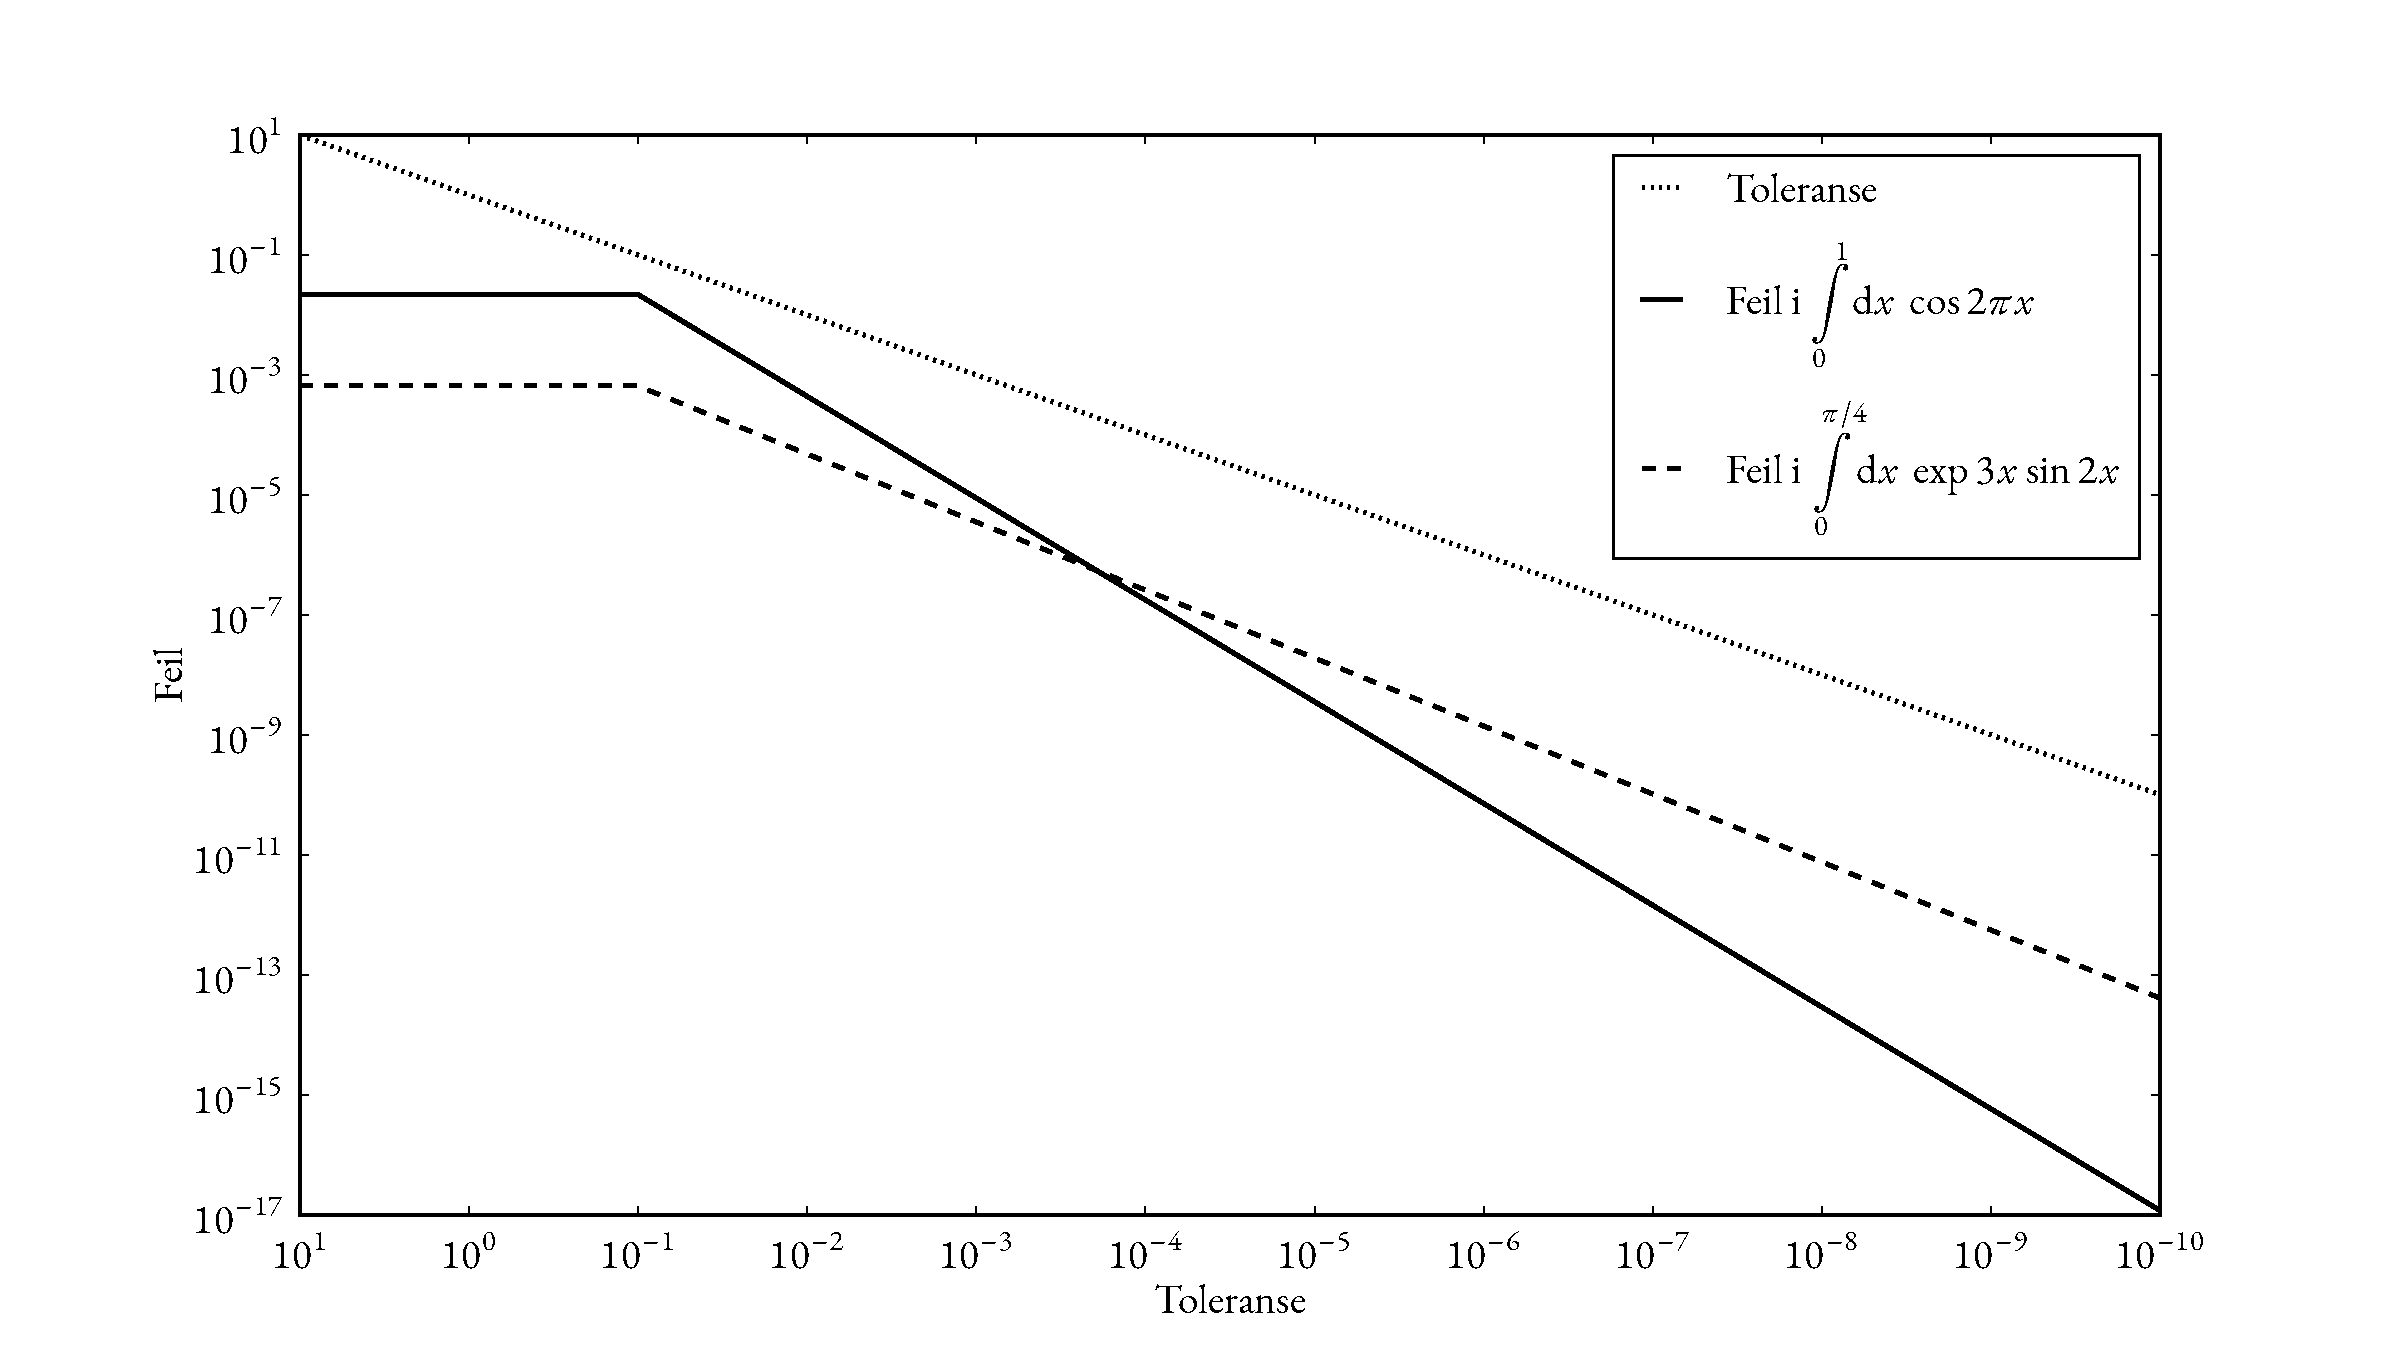
\includegraphics[width=\columnwidth]{simp_err}
    \caption{Feil i adaptiv Simpson-kvadratur.
    Ein ser at feilen er grensa ovanfrå av toleransen.}
\end{figure}



    \section{Simulasjon av fri, stiv lekam}
    Vi ønsker å simulere ein {\em fri, stiv lekam},
    med andre ord ein lekam som ikkje lar seg deformere,
    som roterer fritt i rommet frå ein gitt start-tilstand.

    Fri rotasjon betyr at netto påført dreiemoment er null.
    At lekamen ikkje lar seg deformere medfører at
    treighetsmomentet er konstant. (massen flyttar seg ikkje relativt
    til rotasjons-aksen)
    Dette betyr at normen til dreieimpulsen, og rotasjonsenergien er bevart. \cite{lien}
    Ingenting hindrar dreieimpulsen i å endre retning.

    \subsection{Definisjon av problemet}
    Differensiallikninga
    \cite[Namn på symbola er endra for å passe vår oppgåvetekst]{lien}
    \begin{equation}
        \Mat T \deldel{\vec \upomega}{t} + \vec \upomega \times \Mat T\vec \upomega = \Mat M
        \label{_euler}
    \end{equation}
    skildrar rotasjonen til eit stivt legeme.
    Her er $\Mat M$ påført dreiemoment,
    $\Mat T$ treighetsmoment, og $\vec \upomega$ vinkelfart.
    Per antagelse er $M = 0$. Innfør substitusjonen
    \[
        \vec m = \Mat T \vec \upomega
    \]
    \[
        \implies \deldel{\vec m}{t} = \Mat T \dd{\upomega}{t} \quad\text{og} \quad
        \vec \upomega = \Mat T^{-1} \vec m
    \]
    i \eqref{_euler},
    trekk frå $\textdd{\vec m}{t}$ på begge sider,
    og snu kryss-produktet for å få like forteikn.
    Samtidig innfører vi notasjonen $\dot f = \textdd{f}{t}$.
    \begin{equation}
        \dot \vec m = \vec m \times \Mat T^{-1} \vec m
        \label{euler}
        \tag{\ref{_euler}*}
    \end{equation}
    Bevaringslovene nevnt til å byrje med gir oss:
    \begin{align}
        \label{sph}
        \gamma &= \Norm{\vec m}^2 = \vec m(t) \cdot \vec m(t) \\
        \label{ell}
        E &= \frac{1}{2} \vec m(t) \cdot \Mat T^{-1} \vec m(t)
    \end{align}
    Der \eqref{sph} er ei sfære med radius  $\Norm{\vec m}$,
    og \eqref{ell} er ei ellipse.
    Sidan både $\gamma$ og $E$ er konstantar er løysingane $\vec m$ begrensa
    til å sitje på skjæringa mellom flatene.

    %% $\mathscr J$
    Anta $\Mat T = \Diag(\Mat I_1, \Mat I_2, \Mat I_3)$.
    Ettersom $\Mat T$ er diagonal er
    $\Mat T^{-1} = \Diag(1/\Mat I_1, 1/\Mat I_2, 1/\Mat I_3)$.
    Skriv $\vec m = (x \; y \; z)$, og skriv ut \eqref{euler}
    på komponentform:
    \begin{align*}
        \underset{\dot \vec m}{\begin{pmatrix}
            \dot x(t) \\ \dot y(t) \\ \dot z(t)
        \end{pmatrix}}
        =
        \underset{\vec m}{\begin{pmatrix}
            x(t) \\ y(t) \\ z(t)
        \end{pmatrix}}
        \times
        \left[
            \underset{\Mat T^{-1}}{\begin{pmatrix}
            1/\Mat I_1 &0&0 \\ 0& 1/\Mat I_2 &0 \\ 0&0& 1/\Mat I_3
        \end{pmatrix}}
        \underset{\vec m}{\begin{pmatrix}
            x(t) \\ y(t) \\ z(t)
    \end{pmatrix}}
    \right]
    \end{align*}
    Rekn ut kryssproduktet:
    \begin{align}
        \label{euler_komp}
        \underset{\dot \vec m}{\begin{pmatrix}
            \dot x(t) \\ \dot y(t) \\ \dot z(t)
        \end{pmatrix}}
        =
        \underset{f(t, \vec m)}{\begin{pmatrix}
            A y(t) z(t) \\ B x(t) z(t) \\ C  x(t) y(t)
        \end{pmatrix}}
    \end{align}
    der $A$, $B$ og $C$ er konstantar
    \begin{align*}
        A = 1/I_3 - 1/I_2 \\
        B = 1/I_1 - 1/I_3 \\
        C = 1/I_2 - 1/I_1
    \end{align*}

    \subsection{Implisitt Runge-Kutta midtpunkt-metode}
    Vi ønsker å løyse differensiallikningar av sorten
    \[
        \dot y = f(t, y)
    \]
    numerisk, ved hjelp av Runge-Kutta metoden
    \begin{equation}
        y_{n + 1} = y_n + h f\left( t_n + \frac{h}{2}, \frac{1}{2}(y_n + y_{n + 1})\right) \text,
        \label{mpm}
    \end{equation}
    kalt {\em implisitt midtpunktmetode}, fordi $y_{n+1}$ avheng
    av eit estimat for $y_{n+1/2}$ (derav implisitt)
    for å estimere tangenten i midpunktet mellom $t_n$ og $t_{n+1}$.
    Substituer
    \[
        u = \frac 1 2 (y_n + y_{n + 1}) \implies y_{n+1} = 2u - y_n
    \]
    for å forenkle notasjonen litt.
    Dette gir likningssystemet
    \begin{align*}
                 & 2u - y_n = y_n + h f\left( t + h/2, u \right) \\
        \implies & u = y_n + \frac h 2 f\left( t+h/2, u \right) \\
        \implies & y_n + \frac h 2 f\left( t+h/2, u \right) - u = 0
    \end{align*}
    som må løysast med omsyn til $u$ for kvart tidssteg.
    Gitt ein verdi for $u$ reknar vi ut $y_{n+1}$:
    \begin{equation}
        y_{n+1} = y_n + h f(t + h/2, u)
    \end{equation}

    \subsection*{Anvending på problemet}
    Eitt steg gjenstår før vi kan implementere løysaren:
    Vi er nøtt å velgje ein måte å løyse det implisitte steget.
    Frå \eqref{euler} får vi, med $\vec u = (x \, y \, z)$, likninga
    \begin{equation}
        \label{u_eq}
        \vec F (\vec u) =
        \begin{pmatrix}
            x_n \\ y_n \\ z_n
        \end{pmatrix}
        + \frac h 2
        \begin{pmatrix}
            A y z \\ B x z \\ C x y
        \end{pmatrix}
        -
        \begin{pmatrix}
            x \\ y \\ z
        \end{pmatrix}
        = 0 \text.
    \end{equation}
    Vi innlemmer $h/2$ i konstantane $A$, $B$ og $C$.
    Til slutt sit vi att med systemet
    \begin{align*}
        \left\{
        \begin{array}{c}
            x_n + \hat A y z - x = 0 \\
            y_n + \hat B x z - y = 0 \\
            z_n + \hat C x y - z = 0
        \end{array}
        \right.
    \end{align*}
    der $x_n$, $y_n$, $z_n$,
    samt $\hat A$, $\hat B$ og $\hat C$ er kjende konstantar.
    Jacobian-matrisa lar seg enkelt rekne ut ved hjelp av symbolske
    verktøy, til dømes {\tt sympy} i Python. Vi har
    \[
        \mathscr J_\vec F = \begin{pmatrix}
            -1          &   \hat A z    & \hat A y \\
            \hat B z    &   -1          & \hat B x \\
            \hat C y    &   \hat C x    & -1
        \end{pmatrix} \text.
    \]
    Altso kan vi finne $\vec u = (x \; y\; z)$ med å bruke Newtons metode:
    \[
        \vec u \longleftarrow \vec u - \mathscr J^{-1}_\vec F \vec F(\vec u)
    \]
    som burde konvergere i løpet av svært få iterasjonar dersom vi brukar
    førre iterasjon som startpunkt, og relativt kort skrittlengde.


    \subsection{Implementasjon av RK-metoden}
    Vi brukar eit symbolsk verktøy for å rekne ut \eqref{u_eq}
    i forkant; koden for dette er ikkje spesielt vanskelig,
    men den er stygg, så eg har klipt den ut.
    Den kan finnast i notebooken {\tt rk3d.pynb}.

\begin{python}[caption={Implisitt Runge-Kutta midtpunktmetode.}]
def RK(f, y0, t):

# (sympy-junk removed from here)
# F = F(u), Ji = inv(Jac(F))

y = np.empty((len(t), 3))
y[0] = y0

for n in range(len(t) - 1):
    h = t[n + 1] - t[n]

    u = newton(
        lambda u:  F(u, y[n], t[n] + h/2, h),
        lambda u: Ji(u, y[n], t[n] + h/2, h),
        y[n]
    )

    m = np.array(f(t[n] + h/2, u), dtype=float)

    y[n + 1] = y[n] + h * m

return y.T
\end{python}
I metoden inngår Newtons metode;
denne har vi implementert i ei tidlegare øving,
men legg den ved for kompletthets skuld:
\begin{python}[caption={Newtons metode frå tidlegare øving.}]
def newton(F, Ji, u0, tol=1e-10, maxiter=10):
    u = u0
    for _ in range(maxiter):
        u = u - Ji(u).dot(F(u))

        if linalg.norm(F(u)) < tol:
            break

    return u
\end{python}
Den eine haka ved implementasjonen er at differensiallikninga vi
vil løyse, for det første, må vera tredimensjonell,
og for det andre må vera definert berre ved hjelp av
funksjonar som er kompatible med {\tt sympy}.

Desse vala er gjort med vilje;
det er enklare å ha eit eksplisitt uttrykk for
Jacobian-matrisa ved kvart tidssteg, (som ein får ved å rekne den ut i forkant)
enn å forsøke å estimere den numerisk.
Når ein har bestemt seg for å bruke symbolske metodar
i staden for tilnærmingar er det enklare å
behandle uttrykk der dimensjonen er kjend.
{\tt sympy} {\em har} funksjonalitet for å lage
vektorar med symbol, så det er (i prinsippet) mogleg,
men element i desse vektorane får obskure navn (som ``{\tt \_dummy\_123}'')
som gjer feilsøking til eit mareritt.

\begin{figure}[H]
    \centering
    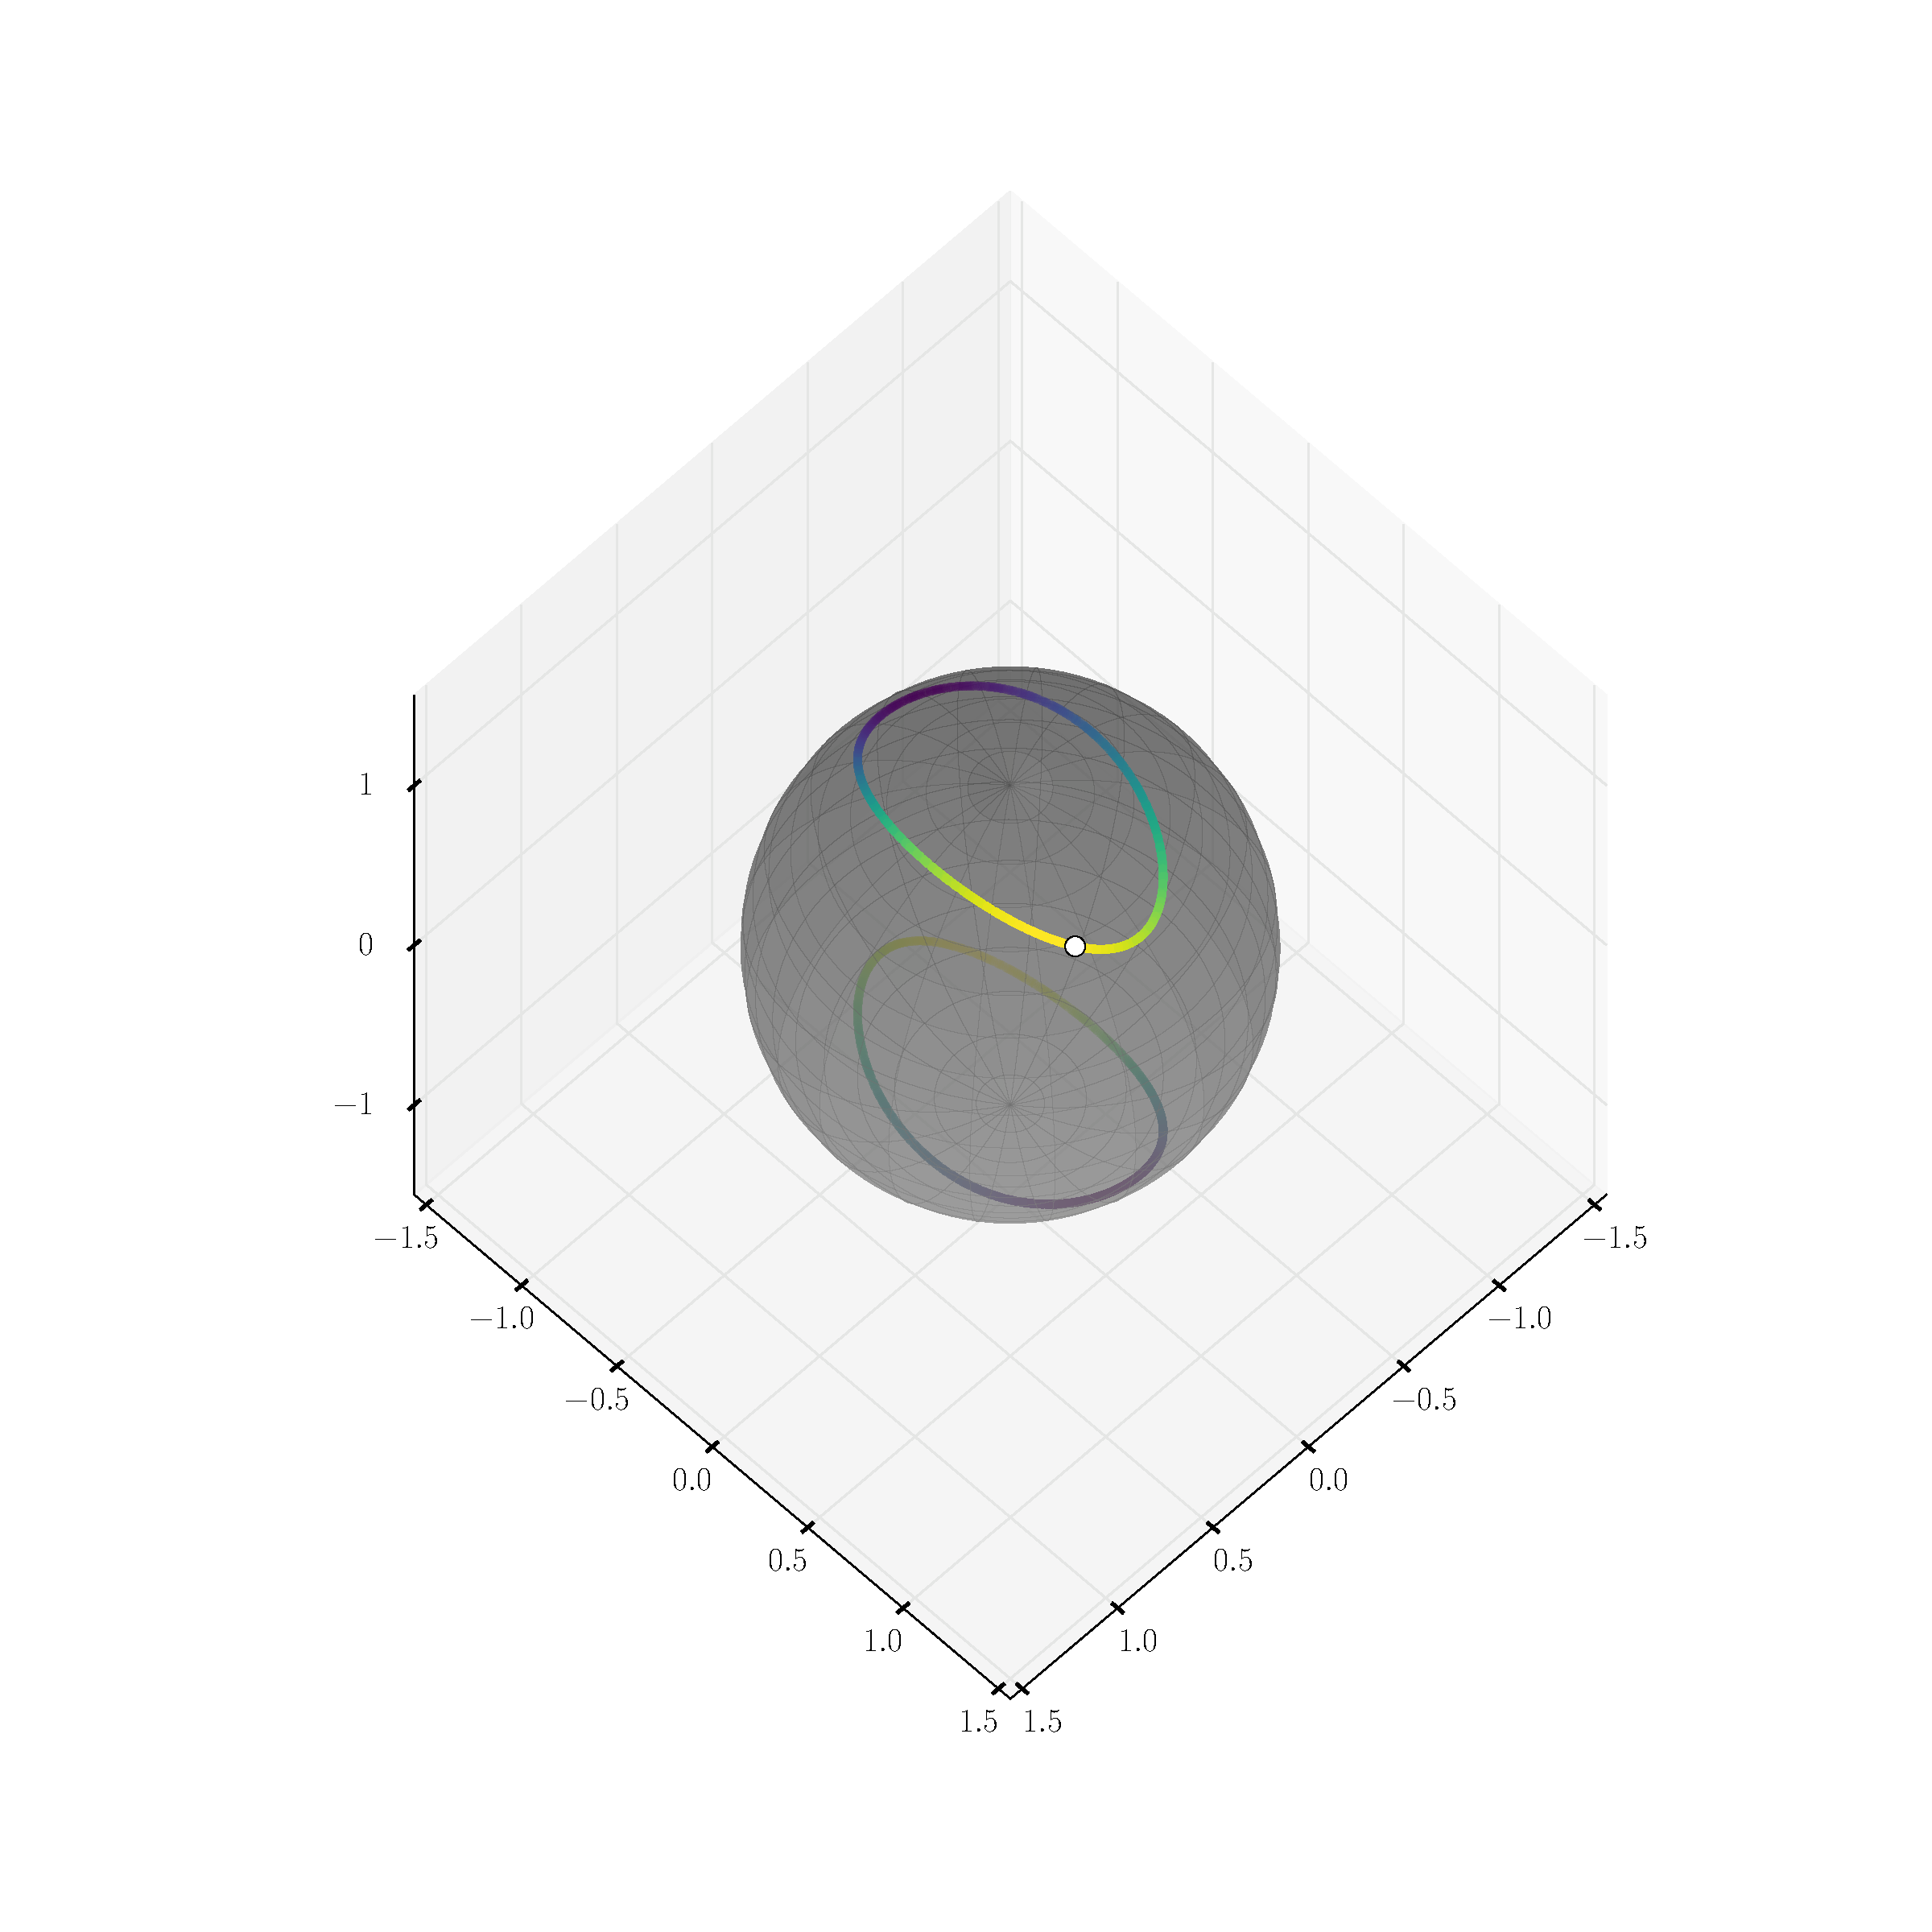
\includegraphics[width=\columnwidth]{euler}
    \caption{
        Løysing av \eqref{euler} med initialverdiar
        $T = \Diag(1, 2, 5)$ og $m_0 = (2 \; 5 \; 7)$.
        Tidsrommet er $[t = 0,\; t = 250]$, med $N = 500$ steg
        med lik steglengde.
        Motsette punkt på sfæra er farga likt,
        $m_0$ er farga kvitt.
    }
\end{figure}







    \printbibliography


\end{multicols*}
\end{document}
